\documentclass{article}
%\input longdiv.tex
\usepackage{amsfonts}
\usepackage{amsmath}
\usepackage{mathtools}
\usepackage{systeme}
\usepackage{polynom}
\usepackage{pgfplots}
\DeclarePairedDelimiter\ceil{\lceil}{\rceil}
\begin{document}
\begin{center}
\Large\textbf{Kodut\"o\"o nr. 4}\\
10. variant\\
\small{Joosep N\"aks}
\end{center}
\textbf{1.} Leidke piirv\"a\"artus, t\~olgendades seda sobivalt valitud funktsiooni integraalsummade piirv\"a\"artusnea:
\begin{gather*}
\lim_{n\to\infty}\left(\frac{1}{n+1}+\frac{1}{n+2}+...+\frac{1}{3n}\right).
\end{gather*}
\textbf{Lahendus:}
\begin{equation*}
\begin{aligned}
\lim_{n\to\infty}\left(\frac{1}{n+1}+\frac{1}{n+2}+...+\frac{1}{3n}\right)&=\lim_{n\to\infty}\left(\frac{1}{n}\frac{1}{1+\frac{1}{n}}+\frac{1}{n}\frac{1}{1+\frac{2}{n}}+...+\frac{1}{n}\frac{1}{3}\right)\\
&=\lim_{n\to\infty}\frac{1}{n}\left(\frac{1}{1+\frac{1}{n}}+\frac{1}{1+\frac{2}{n}}+...+\frac{1}{3}\right)\\
&=\lim_{n\to\infty}\frac{1}{n}\left(\sum_{k=1}^{2n}\frac{1}{1+\frac{k}{n}}\right)\\
&=\lim_{n\to\infty}\sum_{k=1}^{2n}\frac{1}{1+\frac{k}{n}}\frac{1}{n}\\
\end{aligned}
\end{equation*}
Saadud summas on funktsioon $f(x)=\frac{1}{x}$, kus argumendi samm on $\frac{1}{n}$, mis l\"aheneb 0le, ning see on ka l\"abi korrutatud $\frac{1}{n}$ga, nii et see on funktsiooni $f(x)$ integraalsumma, kus k\~oik alamjaotuse l\~oigud l\"ahenevad 0le. Seega on see definitsiooni j\"argi Riemanni integraal l\~oigus $[1,3]$:
\begin{equation*}
\begin{aligned}
&=\int_1^3\frac{1}{x}dx\\
&=\ln(x)|_1^3\\
&=\ln(3)-\ln(1)\\
&=\ln(3)
\end{aligned}
\end{equation*}
\pagebreak\\
\textbf{2.} Leidke piirv\"a\"artus
\begin{gather*}
\lim_{x\to\infty}\frac{1}{x^2}\int_0^x\ln\frac{2t^3}{t^2+1}dt.
\end{gather*}
\textbf{Lahendus:} Vaatlen funktisooni $f(t)=\ln\frac{2t^3}{t^2+1}$. V\~otan sellest tuletise:
\begin{equation*}
\begin{aligned}
f'(t)&=\frac{t^2+1}{2t^3}*\frac{6t^2(t^2+1)-2t^3*2t}{(t^2+1)^2}\\
&=\frac{3(t^2+1)-2t^2}{t(t^2+1)}\\
&=\frac{t^2+3}{t(t^2+1)}
\end{aligned}
\end{equation*}
Kuna saadud tuletis on positiivse argumendi puhul positiivne, on funktsioon $f$ rangelt kasvav positiivse sisendi puhul. Kehtib $f(1)=0$, seega kuna $f$ on rangelt kasvav, on $f$ positiivne vahemikus $[1,\infty)$. Kuna funktsioon $f$ on selles vahemikus positiivne ja rangelt kasvav, on tema integraal selles vahemikus $\infty$.
Vahemikus $(0,1]$ funktsiooni siseminel osal kehtib $\frac{2t^3}{t^2+1} \geq \frac{2t^3}{2}$ kuna $t^2+1$ muutub vahemikus $(1,2]$. Funktsioon $\ln(x)$ on rangelt kasvav funktsioon, seega kehtib ka $\ln\frac{2t^3}{t^2+1} \geq \ln\frac{2t^3}{2}$ ning integraali monotoonsuse p\~ohjal kehtib ka v\~orratus $\int_0^1\ln\frac{2t^3}{t^2+1}\ dt \geq \int_0^1\ln\frac{2t^3}{2}\ dt$. Leian selle integraali:
\begin{equation*}
\begin{aligned}
\int_0^1\ln\frac{2t^3}{2}dt&=\int_0^13\ln t\ dt\\
&=3t(\ln t-1)|_0^1\\
&=3(1(\ln 1-1)-(\lim_{x\to0}x\ln x-x))\\
&=3(-1-\lim_{x\to0}\frac{\ln x}{\frac{1}{x}})\qquad \text{(Kasutan\ l'H\^ospitali\ reeglit)}\\
&=3(-1-\lim_{x\to0}\frac{\frac{1}{x}}{\frac{-1}{x^2}})\\
&=3(-1-\lim_{x\to0}(-x))\\
&=3(-1-0)\\
&=-3
\end{aligned}
\end{equation*}
Seega integraali aditiivsuse kohaselt on funktsiooni $f$ integraal vahemikus $(0,\infty)$ selline:
\begin{equation*}
\begin{aligned}
\int_0^\infty\ln\frac{2t^3}{t^2+1}dt&=\int_0^1\ln\frac{2t^3}{t^2+1}\ dt+\int_0^1\ln\frac{2t^3}{t^2+1}\ dt\geq\\
&\geq \int_0^1\ln\frac{2t^3}{2}\ dt+\int_1^\infty\ln\frac{2t^3}{t^2+1}\ dt\\
&=-3+\infty\\
&=\infty
\end{aligned}
\end{equation*}
Vaatlen n\"u\"ud algset piirv\"a\"artust $\displaystyle\lim_{x\to\infty}\frac{1}{x^2}\int_0^x\ln\frac{2t^3}{t^2+1}dt$. Kuna $\displaystyle\int_0^\infty\ln\frac{2t^3}{t^2+1}dt=\infty$, saab siin kasutada l'H\^osptiali reeglit. Diferentsiaal-integraalarvutuse p\~ohiteoreemi kohaselt kehtib $\displaystyle\frac{d}{dx}\left(\int_0^x\ln\frac{2t^3}{t^2+1}dt\right)=\ln\frac{2x^3}{x^2+1}$. Leian piirv\"a\"artuse:
\begin{equation*}
\begin{aligned}
\lim_{x\to\infty}\frac{\int_0^x\ln\frac{2t^3}{t^2+1}dt}{x^2}&=\lim_{x\to\infty}\frac{\ln\frac{2x^3}{x^2+1}}{2x}\qquad\text{(Kasutan l'H\^ospitali reeglit)}\\
&=\lim_{x\to\infty}\frac{\frac{x^2+3}{x(x^2+1)}}{2}\qquad\text{(Lugeja tuletise leidmine on juba varem n\"aidatud)}\\
&=\lim_{x\to\infty}\frac{x^2+3}{2x^3+2x}\qquad\text{(Kasutan l'H\^ospitali reeglit)}\\
&=\lim_{x\to\infty}\frac{2x}{6x^2+2}\qquad\text{(Kasutan l'H\^ospitali reeglit)}\\
&=\lim_{x\to\infty}\frac{2}{12x}\\
&=0
\end{aligned}
\end{equation*}
Seega on see piirv\"a\"artus 0.
\pagebreak\\
\textbf{3.} Leidke joontega
\begin{gather*}
y=x^3-2x^2+5,\quad y=x^2+4x-7
\end{gather*}
piiratud tasandilise kujundi pindala.\\
\textbf{Lahendus:} Leian joonte l\~oikepunktid:
\begin{equation*}
\begin{aligned}
x^3-2x^2+5&=x^2+4x-7\\
x^3-3x^2-4x+12&=0\\
\end{aligned}
\end{equation*}
Jagan selle pol\"unoomi $x-2$ga l\"abi:
\begin{equation*}
\begin{aligned}
\frac{x^3-3x^2-4x+12}{x-2}&=x^2-x-6\\
&=(x-3)(x+2)\\
\end{aligned}
\end{equation*}
Seega on nullkohad 2, 3 ja -2. Seega tekib joonte vahele kaks kinnist kujundit.\\
Kujundid joonisel:\\
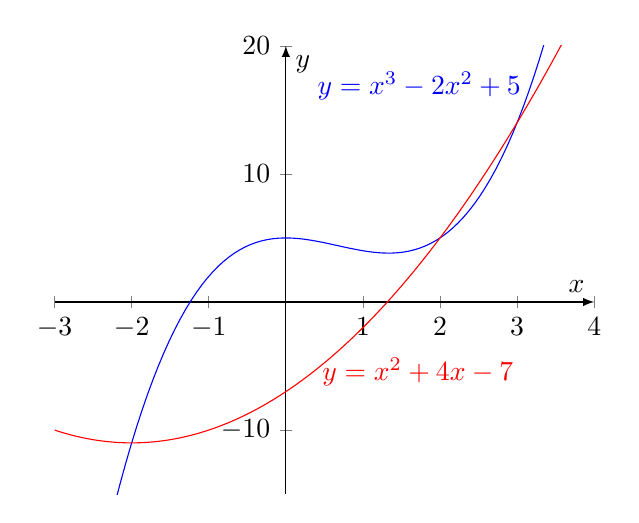
\begin{tikzpicture}
    \begin{axis}[xmin=-3,xmax=4, ymin=-15,ymax=20, axis x line=middle, axis y line=middle, axis line style=-latex, xlabel={$x$}, ylabel={$y$}]
        \addplot [no marks,blue] expression[domain=-3:4,samples=100]{x^3-2*x^2+5} 
                    node[pos=0.75,anchor=east]{$y=x^3-2x^2+5$};
        \addplot [no marks,red] expression[domain=-3:4,samples=100]{x^2+4*x-7}
                                node[pos=0.2,anchor=west]{$y=x^2+4x-7$};
    \end{axis}
\end{tikzpicture}\\
Leian nende pindalad:
\begin{equation*}
\begin{aligned}
S_1&=\left|\int_{-2}^2x^3-2x^2+5\ dx-\int_{-2}^2x^2+4x-7\ dx\right|\\
&=\left|\int_{-2}^2x^3-3x^2-4x+12\ dx\right|\\
&=\left|\left(\frac{1}{4}x^4-\frac{3}{3}x^3-\frac{4}{2}x^2+12x\right)_{-2}^2\right|\\
&=\left|\left(\frac{1}{4}2^4-2^3-2*2^2+12*2\right)-\left(\frac{1}{4}(-2)^4-(-2)^3-2*(-2)^2+12*(-2)\right)\right|\\
&=\left|\left(4-8-8+24\right)-\left(4+8-8-24\right)\right|\\
&=\left|-16+48\right|=32\\
S_2&=\left|\int_2^3x^3-2x^2+5\ dx-\int_2^3x^2+4x-7\ dx\right|\\
&=\left|\int_2^3x^3-3x^2-4x+12\ dx\right|\\
&=\left|\left(\frac{1}{4}x^4-\frac{3}{3}x^3-\frac{4}{2}x^2+12x\right)_2^3\right|\\
&=\left|\left(\frac{1}{4}3^4-3^3-2*3^2+12*3\right)-\left(\frac{1}{4}2^4-2^3-2*2^2+12*2\right)\right|\\
&=\left|\left(\frac{81}{4}-27-18+36\right)-\left(4-8-8+24\right)\right|\\
&=\left|\frac{81}{4}-21\right|=\frac{3}{4}
\end{aligned}
\end{equation*}
Antud joontega kujundite pindalad on 32 ja $\frac{3}{4}$.\\
\end{document}